\chapter{Desenvolvimento}
\label{chap:development}

Esta seção se dedica a descrever como realizar uma implementação utilizando
\textit{WebAssembly}. Para tanto, foi definida uma prova de conceito que consiste em uma
aplicação simples com a finalidade de mensurar a performance entre \textit{WebAssembly} e
\textit{JavaScript}, para que posteriormente seja possível realizar uma análise
comparativa entre os tempos de execução de algoritmos escritos em \textit{WebAssembly} e
\textit{JavaScript} utilizando o método \textit{StopWatch}.

Essa aplicação foi construída utilizando as três principais linguagens suportadas pelos
navegadores até então: \textit{HTML}, \textit{CSS} e \textit{JavaScript}. Entretanto para
a análise de desempenho foram construídos alguns algoritmos utilizando as linguagens
\textit{JavaScript} e \textit{C}, para que pudesse ser feita a comparação entre ambas as
execuções. Todos os testes foram realizados utilizando o navegador \textit{Google Chrome},
que utiliza o motor \textit{JavaScript V8}, e os algoritmos escritos em \textit{C} foram
compilados para a representação binária de \textit{WebAssembly} utilizando o compilador
\textit{Emscripten}.

Para a análise de desempenho foi utilizado o método \textit{StopWatch} que consiste em
medir o tempo decorrido entre o início e fim de uma tarefa. Para facilitar a compreensão
deste método, um exemplo de utilização desta técnica pode ser visto no Código-fonte
\ref{alg:code-6}.

\lstinputlisting[language=JavaScript,caption={\label{alg:code-6} Exemplo de utilização da técnica \textit{StopWatch}}]{code/stop_watch.js}

No código acima, pode-se ver que primeiro é obtido o tempo de início da tarefa antes de
executá-la, utilizando o método \textit{now} do objeto \textit{performance}, fornecido
pelo motor JavaScript, que retorna o tempo decorrido desde a criação do contexto de
uma página, em milissegundos. Logo em seguida, é executada a tarefa, através da função
\textit{task}, no exemplo citado. Posteriormente, é obtido o tempo final da tarefa,
utilizando novamente o método \textit{now} do objeto \textit{performance}, e logo depois,
é feita a subtração desses valores, obtendo então o tempo decorrido da execução da tarefa
em questão.

\section{Execução dos algoritmos}
\label{ssec:algorithms-execution}

Para a execução dos testes, foram selecionados 3 algoritmos, eles foram utilizados para
realizar uma análise simples sobre a execução de códigos escritos em \textit{JavaScript} e
\textit{WebAssembly}. São eles:

\begin{itemize}
    \item N-ésimo termo da sequência \textit{Fibonacci}
    \item \textit{ShellSort}
    \item \textit{QuickSort}
\end{itemize}

Para a execução dos algoritmos foram criados alguns objetos, com funções que simplificam
a manipulação dos algoritmos durante suas execuções. Entretanto, serão explicados mais
profundamente apenas os três principais objetos, selecionados devido sua importância
para a aplicação. Os objetos são:

\begin{itemize}
    \item \textit{Benchmark}
    \item \textit{Arrays}
    \item \textit{Runner}
\end{itemize}

O primeiro objeto, \textit{Benchmark}, foi o responsável por implementar a técnica
\textit{StopWatch} na aplicação, foi através dele que foi obtido o tempo decorrido de cada
algoritmo executado. Entretanto, ele não se limita apenas ao tempo de execução, sendo
responsável também por informar o resultado de cada algoritmo. A implementação desse
objeto pode ser vista no Código-fonte \ref{alg:code-7}.

\lstinputlisting[language=JavaScript,caption={\label{alg:code-7} Objeto \textit{Benchmark} utilizado na execução dos testes}]{code/benchmark.js}

O objeto \textit{Benchmark}, possui apenas uma única função, que recebe como parâmetro
o algoritmo a ser executado e retorna dois valores: o tempo decorrido e o resultado dessa
tarefa.

O segundo objeto, \textit{Arrays}, foi utilizado para realizar uma validação simples no
resultado de cada algoritmo: verificar se o resultado obtido através da implementação
em \textit{JavaScript} e \textit{WebAssembly} foi o mesmo. Esse objeto fazendo apenas
essa checagem, foi responsável por verificar quaisquer falha de manipulação de memória
que pudesse nos retornar um resultado falso positivo. A implementação desse objeto pode
ser vista no Código-fonte \ref{alg:code-8}.

\lstinputlisting[language=JavaScript,caption={\label{alg:code-8} Objeto \textit{Arrays} utilizado na execução dos testes}]{code/arrays.js}

O objeto \textit{Arrays} possui apenas uma única função, assim como o objeto
\textit{Benchmark}, que aceita dois vetores como parâmetro e retorna um valor do tipo
\textit{Boolean}, informando se os dois vetores possuem os mesmo valores ou não.

Da linha 2 a linha 4 são realizadas as validações mais simples, onde é verificado se um
dos dois vetores não possui valor, sendo retornado o valor verdadeiro em caso positivo e
falso em caso negativo. Como \textit{JavaScript} possui avaliação de curto-circuito, em
que os argumentos posteriores são avaliados apenas se os argumentos anteriores não forem
suficientes para determinar o valor da expressão, caso seja informado algum vetor vazio,
por exemplo, o motor já identificará nas primeiras condições que os vetores são
diferentes. Na linha 5, é verificado se o tamanho desses vetores é diferente, pois caso
sejam, os vetores em si já serão identificados como diferentes pois não possuem o mesmo
número de elementos. Na linha 6, é utilizado o método \textit{some} para checar elemento
por elemento de ambos os vetores, caso seja identificado em algum índice que os elementos
dos vetores são diferentes a iteração irá parar e será retornado o valor verdadeiro, caso
contrário será retornado o valor falso.

O terceiro objeto, \textit{Runner}, foi o responsável por implementar todo o fluxo de
execução dos algoritmos, manipulando memória quando necessário, gerando os vetores
iniciais que foram utilizados pelos algoritmos de ordenação, verificando o resultado de
cada algoritmo e calculando a relação entre o tempo decorrido entre os algoritmos
implementados em \textit{WebAssembly} e em \textit{JavaScript}. A implementação desse
objeto pode ser vista no Código-fonte \ref{alg:code-9}.

\lstinputlisting[language=JavaScript,caption={\label{alg:code-9} Objeto \textit{Runner} utilizado na execução dos testes}]{code/test_runner.js}

O objeto \textit{Runner} diferente dos dois objetos anteriores, possui três métodos, cada
um responsável pela execução de um algoritmo específico. Dada a importância da compreensão
desses métodos, serão explicados cada um deles individualmente a seguir.

Em cada uma das funções de execução, os parâmetros representam os mesmos objetos,
alterando apenas seus significados de acordo com o algoritmo analisado.

O primeiro parâmetro representa um objeto simples que possui três atributos:

\begin{itemize}
    \item \textit{\textbf{module}}: um objeto que representa a instância do módulo
    \textit{WebAssembly} relacionado ao algoritmo em questão.
    \item \textit{\textbf{wasm}}: uma função escrita em \textit{WebAssembly} relacionada
    ao algoritmo a ser analisado.
    \item \textit{\textbf{js}}: uma função escrita em \textit{JavaScript} relacionada ao
    algoritmo a ser analisado.
\end{itemize}

O segundo parâmetro representa um valor numérico, tendo significados distintos de acordo
com a função de execução.

Esta seção se dedica apenas a explicar a execução de cada um dos algoritmos propostos, e
não os próprios algoritmos em si, com a finalidade de fornecer todos os detalhes sobre
toda a manipulação necessária para a execução dos mesmos, mais detalhes de implementação
de cada uma das duas abordagens, \textit{JavaScript} e \textit{WebAssembly}, serão
explicados e analisados na próxima seção.

\lstinputlisting[language=JavaScript,caption={\label{alg:code-10} Função de execução do algoritmo \textit{Fibonacci}}]{code/fibonacci_test.js}

Iniciando a execução do primeiro algoritmo, seu objetivo é encontrar o n-ésimo termo da
sequência \textit{fibonacci}, sendo o termo a ser encontrado representado pelo segundo
parâmetro da função.

Analisando o código descrito no Código-fonte \ref{alg:code-10}, pode-se ver que nas
linhas 2 e 3, são executados ambos os algoritmos, utilizando o objeto \textit{Benchmark}
já mencionado anteriormente, em que são obtidos os seus resultados e tempos de execução.
Na linha 5 é verificado se os resultados obtidos são diferentes, retornando um valor nulo
caso essa regra seja obedecida, caso contrário a execução do método continua. Na linha 10,
é calculada a relação entre os tempos de execução entre os algoritmos escritos em
\textit{JavaScript} e \textit{WebAssembly}. Na linha 11, são retornados os valores obtidos
de ambas as execuções.

\lstinputlisting[language=JavaScript,caption={\label{alg:code-11} Função de execução do algoritmo \textit{ShellSort}}]{code/shellsort_test.js}

\textit{ShellSort} é um algoritmo de ordenação, de complexidade quadrática, que na
aplicação citada anteriormente, tem como objetivo colocar os elementos dos vetores em
ordem ascendente, ou seja, do elemento de menor valor para o de maior valor, sendo o
tamanho do vetor representado pelo segundo parâmetro da função.

Analisando o código descrito no Código-fonte \ref{alg:code-11}, pode-se ver que da linha 2
a linha 7 são gerados dois vetores de mesmo tamanho e mesmo valores, que serão utilizados
posteriormente. Na linha 9, foi criada uma variável representando a quantidade de
\textit{bytes} ocupados por um tipo flutuante, em \textit{WebAssembly} tipos flutuantes
podem ser de 32 ou 64 \textit{bits}, e como no algoritmo escrito em \textit{C} foi
utilizado o tipo \textit{double}, que em \textit{C} representa 64 \textit{bits}, quando
for gerada a representação binária do algoritmo, utilizando o \textit{Emscripten}, essas
mesmas variáveis de tipo \textit{double} serão representadas com 64 \textit{bits} em
\textit{WebAssembly}, por isso foi atribuído o valor 8 a essa variável representando os 8
\textit{bytes}. Na linha 10, foi criada uma variável para conter o último índice desses
vetores, que será utilizado posteriormente. Na linha 11, é utilizado o método
\textit{\_malloc} para alocar a memória necessária para os elementos do vetor "a" que será
passado para o código \textit{WebAssembly} posteriormente, ocupando 8 \textit{bytes}
por elemento do vetor. Na linha 12, é criada uma variável responsável por conter a
quantidade de deslocamento de \textit{bytes}, de acordo com a quantidade de \textit{bytes}
por elemento do vetor. Na linha 14, é utilizado o campo \textit{HEAPF64} que representa a
\textit{heap} responsável por armazenar campos flutuantes de 64 \textit{bits}. Abaixo
segue uma tabela de mapeamento, de que \textit{heap} utilizar com base em que tipo de
dado:

\begin{table}[ht]
    \Caption{\label{tab:heap} Tabela de mapeamento de \textit{Heap} para o tipo específico}
    \IBGEtab{}{
    \begin{tabular}{ccc}
        \toprule
        Heap & C++ & JavaScript \\
        \midrule \midrule
        HEAP8 & int8\_t & Int8Array \\
        HEAPU8 & uint8\_t & Uint8Array \\
        HEAP16 & int16\_t & Int16Array \\
        HEAPU16 & uint16\_t & Uint16Array \\
        HEAP32 & int32\_t & Int32Array \\
        HEAPU32 & uint32\_t & Uint32Array \\
        HEAPF32 & float & Float32Array \\
        HEAPF64 & double & Float64Array \\
    \end{tabular}
    }{
    \Fonte{Elaborado pelo autor.}
    }
\end{table}

Conforme explicado anteriormente, \textit{WebAssembly} utiliza uma memória linear, que
pode ser entendida como um simples vetor de elementos. Na tabela acima, pode-se ver que
tipo de vetor é utilizado em \textit{JavaScript} na implementação do \textit{WebAssembly}
para armazenar que tipo de dados. Até o momento, cada tipo de dado possui sua própria
\textit{heap}.

Continuando na linha 14, os dados são copiados do vetor para a \textit{heap}, de forma
que o código \textit{WebAssembly} possa manipulá-lo. Na linha 15, é executada a função em
\textit{WebAssembly} referente ao algoritmo \textit{ShellSort}, passando como parâmetro
para a função, a variável representando um ponteiro para o vetor, e o tamanho do vetor.
Na linha 16, são obtidos os valores que estão na \textit{heap} e são atribuídos de volta
ao vetor "a". Na linha 17, é removido da memória o espaço alocado anteriormente, dado
que não será utilizado posteriormente.

\lstinputlisting[language=JavaScript,caption={\label{alg:code-12} Função de execução do algoritmo \textit{QuickSort}}]{code/quicksort_test.js}

A implementação da função de execução do algoritmo \textit{QuickSort} é semelhante a
função do \textit{ShellSort}, tendo como única diferença os parâmetros que são passados
para as implementações dos algoritmos, enquanto no \textit{ShellSort} são passados apenas
dois parâmetros, que são o ponteiro para o vetor e o tamanho do vetor, no
\textit{QuickSort} são passados três parâmetros: o ponteiro representando o vetor, o
índice inicial do vetor e o índice final do vetor.

\section{Comparação}
\label{ssec:comparison}

Como descrito na seção anterior, foram selecionados 3 algoritmos para a realização da
análise do tempo de execução, sendo estes escritos nas linguagens \textit{JavaScript} e
\textit{C}:

\begin{itemize}
    \item N-ésimo termo da sequência \textit{Fibonacci}
    \item \textit{ShellSort}
    \item \textit{QuickSort}
\end{itemize}

A análise consiste da implementação desses algoritmos em cada linguagem, para a obtenção
do tempo de execução de cada um individualmente, utilizando a técnica \textit{StopWatch},
alterando apenas os dados de entrada. Todos os testes foram realizados utilizando o
navegador \textit{Google Chrome}, que utiliza o motor \textit{JavaScript V8}, e os
algoritmos escritos em \textit{C} foram compilados para a representação binária de
\textit{WebAssembly} utilizando a ferramenta \textit{Emscripten}.

O primeiro algoritmo a ser analisado foi o responsável por calcular o n-ésimo termo da
sequência \textit{Fibonacci}, para tanto foi utilizada a implementação em
\textit{JavaScript} que pode ser vista no Código-fonte \ref{alg:code-13}.

\lstinputlisting[language=JavaScript,caption={\label{alg:code-13} Algoritmo responsável por calcular o n-ésimo termo da sequência \textit{Fibonacci} em \textit{JavaScript}}]{code/fibonacci.js}

O mesmo algoritmo foi implementado em \textit{C} utilizando recursão e pode ser visto no
Código-fonte \ref{alg:code-14}.

\lstinputlisting[language=C,caption={\label{alg:code-14} Algoritmo responsável por calcular o n-ésimo termo da sequência \textit{Fibonacci} em \textit{C}}]{code/fibonacci.c}

Como foi possível observar nas implementações exibidas nos códigos-fonte \ref{alg:code-13}
e \ref{alg:code-14}, o mesmo algoritmo foi implementado em \textit{JavaScript} e em
\textit{C}, fazendo com que fosse possível obter o tempo decorrido de cada execução
isoladamente. Os tempos obtidos para cada implementação com base no termo a ser
encontrado, pode ser visto na Tabela \ref{tab:time-1}.

\begin{table}[ht]
    \Caption{\label{tab:time-1} Tempos de execução do algoritmo que calcula o n-ésimo termo da sequência \textit{Fibonacci}}
    \IBGEtab{}{
    \begin{tabular}{cccc}
        \toprule
        Termo & JavaScript (ms) & WebAssembly (ms) & Razão (JS / WA) \\
        \midrule \midrule
        5  & 0.11500     & 0.05500    & 2.09091 \\
        10 & 0.01500     & 0.02000    & 0.75000 \\
        15 & 0.16000     & 0.01000    & 16.00000 \\
        20 & 1.20000     & 0.05000    & 24.00000 \\
        25 & 0.82000     & 0.36500    & 2.24658 \\
        30 & 8.63500     & 3.13500    & 2.75439 \\
        35 & 94.79500    & 32.33500   & 2.93165 \\
        40 & 1098.46000  & 360.71000  & 3.04527 \\
        45 & 11907.52500 & 4212.73500 & 2.82655 \\
        \bottomrule
    \end{tabular}
    }{
    \Fonte{Elaborado pelo autor.}
    \Nota[Ambiente]{Teste realizado no navegador \textit{Google Chrome} que utiliza o motor
    \textit{JavaScript V8}.}
    }
\end{table}

Como foi possível perceber, com base na Tabela \ref{tab:time-1}, \textit{WebAssembly} se
mostrou mais eficiente que \textit{JavaScript} em quase todos os casos, com exceção da
execução do algoritmo que busca pelo décimo termo da sequência \textit{Fibonacci}, em que
a execução de \textit{JavaScript} foi de aproximadamente 30\% mais eficiente que a
execução em \textit{WebAssembly}, entretanto, no melhor caso, \textit{WebAssembly}
utilizou apenas aproximadamente 4\% do tempo decorrido pelo mesmo algoritmo escrito em
\textit{JavaScript}, onde buscou-se pelo vigésimo termo da sequência.

O segundo algoritmo trata-se de um algoritmo de ordenação denominado \textit{ShellSort},
que na aplicação proposta tem como objetivo colocar os elementos de um vetor em ordem
ascendente. A implementação feita em \textit{JavaScript} pode ser vista no
Código-fonte \ref{alg:code-15}.

\lstinputlisting[language=JavaScript,caption={\label{alg:code-15} \textit{ShellSort} em \textit{JavaScript}}]{code/shell_sort.js}

A mesma implementação do algoritmo \textit{ShellSort} foi realizada em \textit{C}, e pode
ser visto no Código-fonte \ref{alg:code-16}.

\lstinputlisting[language=C,caption={\label{alg:code-16} \textit{ShellSort} em \textit{C}}]{code/shell_sort.c}

O mesmo algoritmo foi implementado em \textit{JavaScript} e em \textit{C}, e foram obtidos
os seguintes resultados referentes ao tempo de execução e dados de entrada:

\begin{table}[ht]
    \Caption{\label{tab:time-2} Tempos de execução do algoritmo \textit{ShellSort}}
    \IBGEtab{}{
    \begin{tabular}{cccc}
        \toprule
        Tamanho do vetor & JavaScript (ms) & WebAssembly (ms) & Razão (JS / WA) \\
        \midrule \midrule
        10    & 0.10500  & 0.10500 & 1.00000 \\
        100   & 0.06500  & 0.01000 & 6.50000 \\
        1000  & 3.64500  & 0.09500 & 38.36842 \\
        2000  & 1.88500  & 0.20500 & 9.19512 \\
        3000  & 0.38000  & 0.31500 & 1.20635 \\
        4000  & 0.52000  & 0.47000 & 1.10638 \\
        5000  & 0.82000  & 0.67000 & 1.22388 \\
        25000 & 5.00500  & 4.09500 & 1.22222 \\
        50000 & 10.26000 & 8.42000 & 1.21853 \\
        \bottomrule
    \end{tabular}
    }{
    \Fonte{Elaborado pelo autor.}
    \Nota[Vetor]{Itens do vetor gerados aleatoriamente.}
    \Nota[Ambiente]{Teste realizado no navegador \textit{Google Chrome} que utiliza o
    motor \textit{JavaScript V8}.}
    }
\end{table}

Com base na Tabela \ref{tab:time-2}, pode-se observar que a execução do algoritmo escrito
em \textit{WebAssembly} teve performance superior ao escrito em \textit{JavaScript} em
quase todos os casos. No pior caso, o algoritmo em \textit{WebAssembly} utilizou
aproximadamente o mesmo tempo decorrido pelo algoritmo em \textit{JavaScript}, entretanto,
no melhor caso, o algoritmo escrito em \textit{WebAssembly} chegou a utilizar apenas
aproximadamente 3\% do tempo utilizado pelo algoritmo em \textit{JavaScript}, em que foi
utilizado um vetor com 1000 elementos.

O terceiro algoritmo também trata-se de um algoritmo de ordenação, denominado
\textit{QuickSort}, que na aplicação proposta tem como objetivo colocar os elementos de um
vetor em ordem ascendente. A implementação feita em \textit{JavaScript} pode ser vista no
Código-fonte \ref{alg:code-17}.

\lstinputlisting[language=JavaScript,caption={\label{alg:code-17} \textit{QuickSort} em \textit{JavaScript}}]{code/quick_sort.js}

O mesmo algoritmo foi implementado em \textit{C} e pode ser visto no Código-fonte
\ref{alg:code-18}.

\lstinputlisting[language=C,caption={\label{alg:code-18} \textit{QuickSort} em \textit{C}}]{code/quick_sort.c}

O mesmo algoritmo foi implementado em \textit{JavaScript} e em \textit{C}, e foram obtidos
os seguintes resultados referentes ao tempo de execução e dados de entrada:

\begin{table}[ht]
    \Caption{\label{tab:time-3} Tempos de execução do algoritmo \textit{QuickSort}}
    \IBGEtab{}{
    \begin{tabular}{cccc}
        \toprule
        Tamanho do vetor & JavaScript (ms) & WebAssembly (ms) & Razão (JS / WA) \\
        \midrule \midrule
        10       & 0.27000     & 0.06500    & 4.15385 \\
        100      & 0.07500     & 0.01000    & 7.50000 \\
        1000     & 2.37500     & 0.09000    & 26.38889 \\
        10000    & 1.23500     & 1.06500    & 1.15962 \\
        100000   & 15.78000    & 13.14000   & 1.20091 \\
        1000000  & 179.01000   & 160.65500  & 1.11425 \\
        10000000 & 2171.02000  & 1861.00500 & 1.16658 \\
        20000000 & 4224.75500  & 3724.26000 & 1.13439 \\
        30000000 & 6662.29500  & 5761.54500 & 1.15634 \\
        40000000 & 9594.70000  & 7917.12000 & 1.21189 \\
        50000000 & 11478.08000 & 9998.39500 & 1.14799 \\
        \bottomrule
    \end{tabular}
    }{
    \Fonte{Elaborado pelo autor.}
    \Nota[Vetor]{Itens do vetor gerados aleatoriamente.}
    \Nota[Ambiente]{Teste realizado no navegador \textit{Google Chrome} que utiliza o
    motor \textit{JavaScript V8}.}
    }
\end{table}

Analisando a Tabela \ref{tab:time-3}, pode-se observar que o algoritmo escrito em
\textit{WebAssembly} teve tempo de execução superior ao escrito em \textit{JavaScript} em
todos os casos, em que na melhor execução utilizou apenas aproximadamente 4\% do tempo
utilizado pelo mesmo algoritmo escrito em \textit{JavaScript}, onde foi utilizado um
vetor com 1000 elementos.

Com base nos resultados obtidos exibidos nas tabelas \ref{tab:time-1}, \ref{tab:time-2} e
\ref{tab:time-3}, foram gerados os gráficos exibidos nas figuras \ref{fig:image-10},
\ref{fig:image-11} e \ref{fig:image-12}. Esses gráficos possuem 4 dados-chave: os dados
de entrada, o tempo utilizado por ambas as implementações para conclusão da tarefa
proposta e a média de tempo gasto com base nos tempos de execução obtidos.

\begin{figure}[h!]
    \centering
    \Caption{\label{fig:image-10} Resultados do algoritmo que descobre o n-ésimo termo da sequência \textit{Fibonacci}}
    \UECEfig{}{
    \fbox{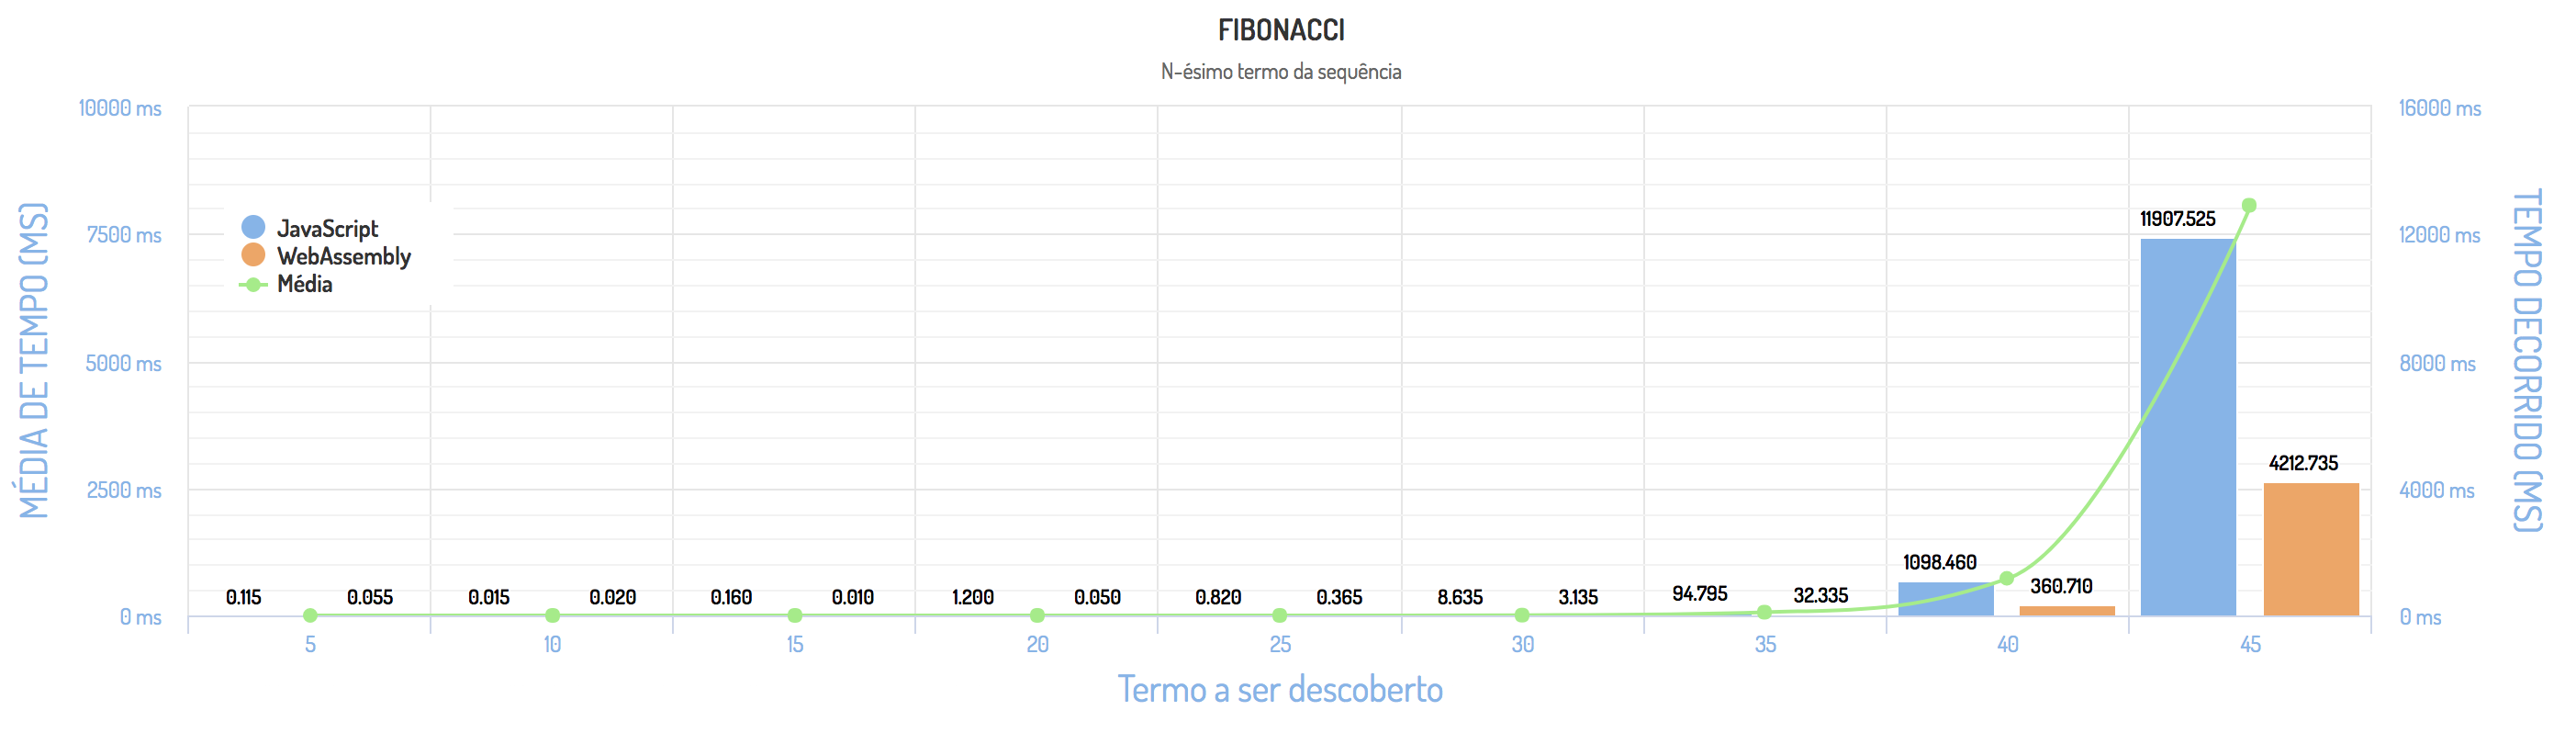
\includegraphics[width=16cm]{graphics/fibonacci}}
    }{
    \Fonte{Elaborada pelo autor.}
    }
\end{figure}

\begin{figure}[h!]
    \centering
    \Caption{\label{fig:image-11} Resultados do algoritmo \textit{ShellSort}}
    \UECEfig{}{
    \fbox{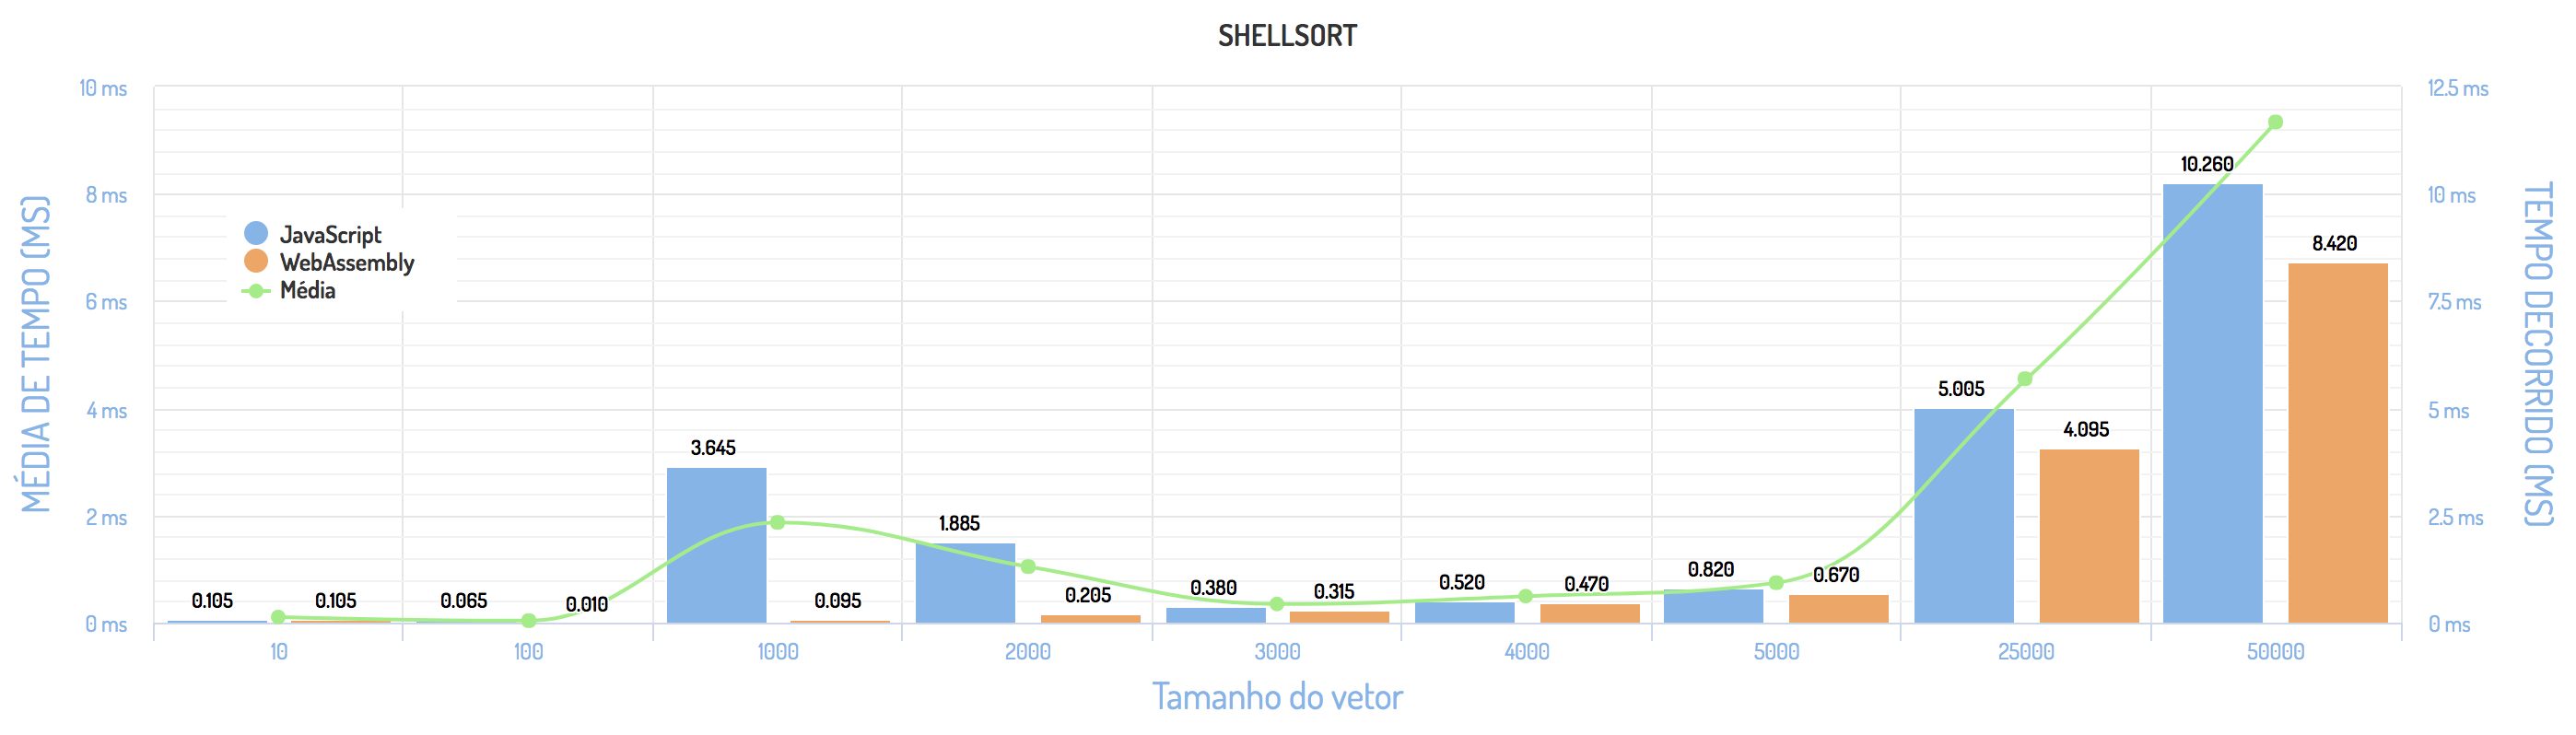
\includegraphics[width=16cm]{graphics/shell_sort}}
    }{
    \Fonte{Elaborada pelo autor.}
    }
\end{figure}

\begin{figure}[h!]
    \centering
    \Caption{\label{fig:image-12} Resultados do algoritmo \textit{QuickSort}}
    \UECEfig{}{
    \fbox{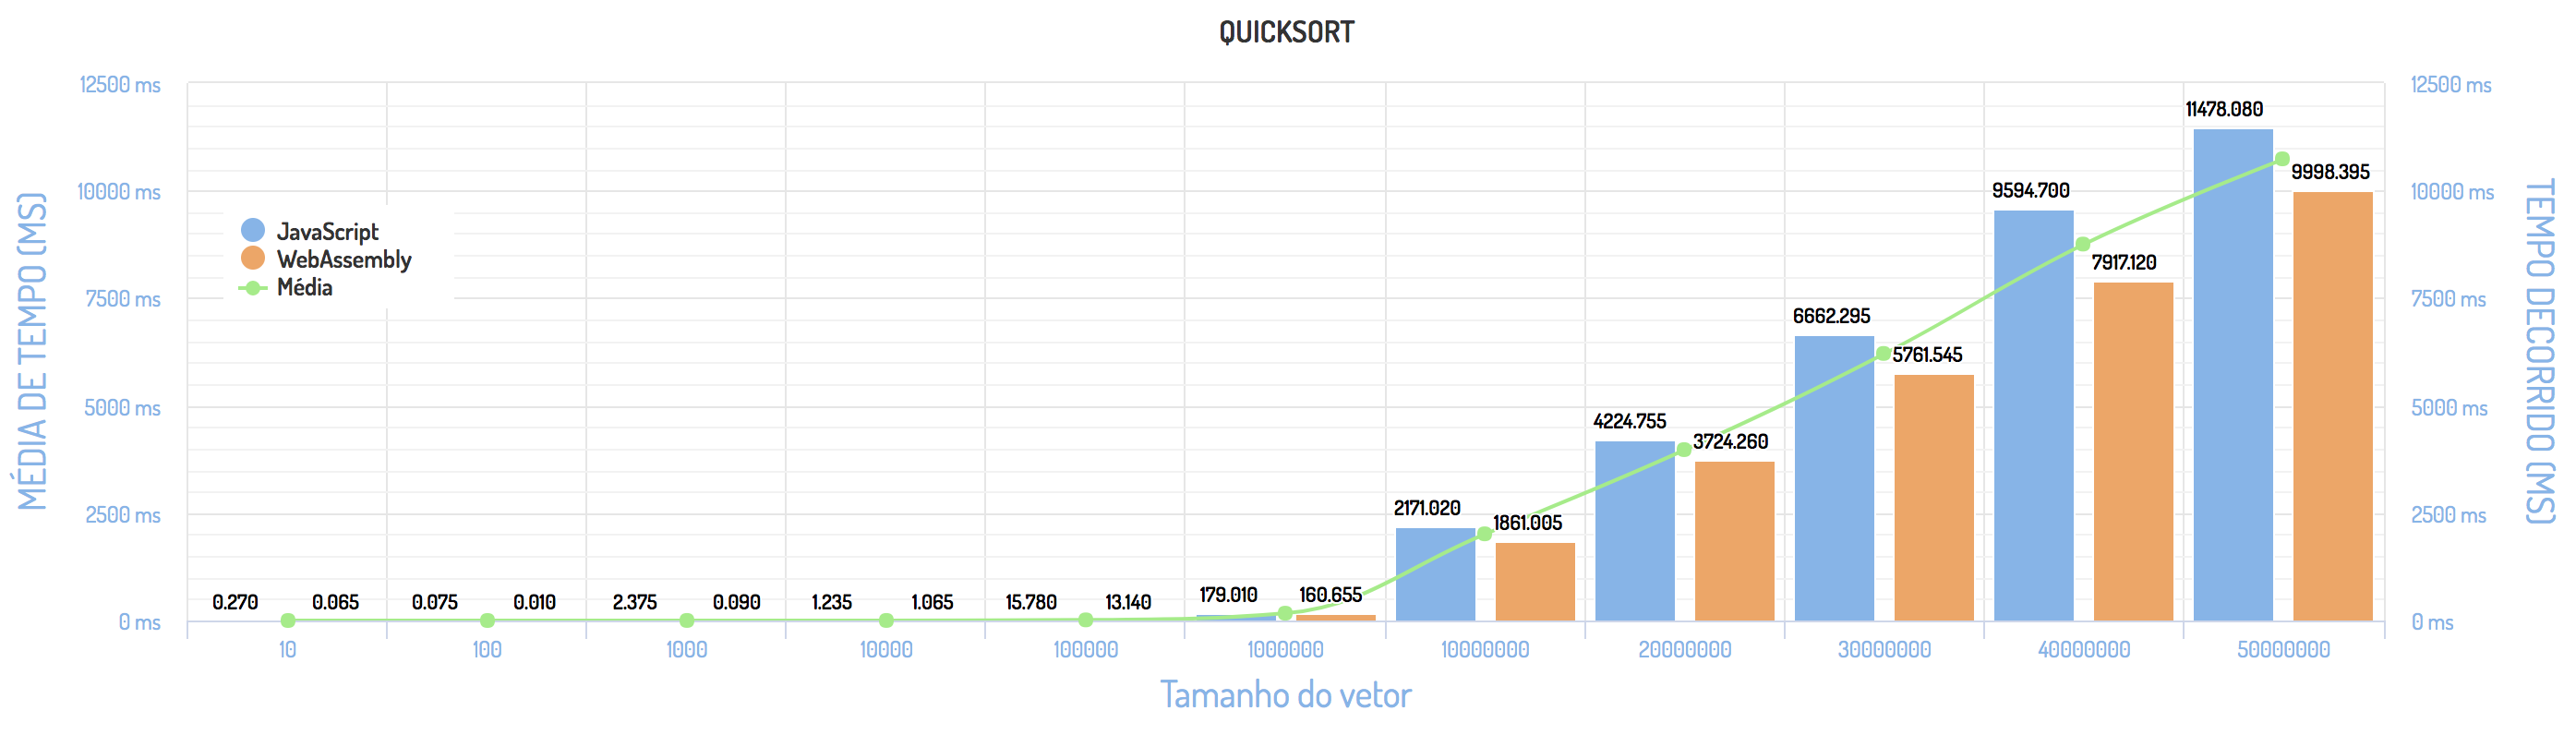
\includegraphics[width=16cm]{graphics/quick_sort}}
    }{
    \Fonte{Elaborada pelo autor.}
    }
\end{figure}

Com base nos resultados exibidos nas figuras \ref{fig:image-10}, \ref{fig:image-11} e
\ref{fig:image-12}, pode-se observar que em quase todos os casos, os algoritmos escritos
em \textit{WebAssembly} tiveram performance superior aos escritos em \textit{JavaScript},
com apenas duas exceções: a primeira, na execução do algoritmo que busca o n-ésimo termo
da sequência \textit{Fibonacci}, em que a implementação escrita em \textit{WebAssembly}
obteve resultado inferior a implementação escrita em \textit{JavaScript}; e a segunda
exceção, obtida na implementação do algoritmo \textit{ShellSort}, em que o algoritmo
escrito em \textit{WebAssembly} obteve aproximadamente o mesmo tempo de execução que o
algoritmo escrito em \textit{JavaScript}.

Em cada algoritmo testado, houveram execuções que apresentaram disparidade bastante
significativa:

\begin{itemize}
    \item \textbf{N-ésimo termo da sequência \textit{Fibonacci}}: na busca pelo vigésimo
    termo da sequência, o tempo utilizado pelo algoritmo escrito em \textit{JavaScript}
    foi de aproximadamente 2300\% superior ao utilizado pelo algoritmo escrito em
    \textit{WebAssembly}.
    \item \textbf{\textit{ShellSort}}: na execução que utilizou um vetor com 1000
    elementos, o tempo utilizado pelo algoritmo escrito em \textit{JavaScript} foi de
    aproximadamente 3700\% superior ao utilizado pelo algoritmo escrito em
    \textit{WebAssembly}.
    \item \textbf{\textit{QuickSort}}: na execução que utilizou um vetor com 1000
    elementos, o tempo utilizado pelo algoritmo escrito em \textit{JavaScript} foi de
    aproximadamente 2500\% superior ao utilizado pelo algoritmo escrito em
    \textit{WebAssembly}.
\end{itemize}

\section{Discussão}
\label{ssec:discussion}

De acordo com o que foi apresentado na seção anterior, é possível perceber que o
desempenho de um algoritmo escrito em \textit{WebAssembly} é na maioria dos casos,
superior ao mesmo algoritmo escrito em \textit{JavaScript}. Isso é devido a sua execução,
enquanto um código escrito em \textit{JavaScript} precisa ser transformado em uma Árvore
de Sintaxe Abstrata e posteriormente convertido em uma representação intermediária, um
código escrito em \textit{WebAssembly} não precisa realizar esses passos, pois ele já é
uma representação intermediária, precisando apenas ser decodificado e verificado para
garantir que não há erros em sua estrutura interna.

Um código escrito em \textit{JavaScript} é compilado durante sua execução, utilizando o
compilador \textit{Just-in-Time}, e dependendo dos tipos que são utilizados em tempo de
execução, múltiplas versões do mesmo código precisam ser compilados utilizando o
compilador de otimização, para garantir que um bloco de código será otimizado
independente dos tipos de dados utilizados internamente, e isso possui um custo elevado
devido ter que monitorar os tipos de dados em execução. Outra observação importante é que
os compiladores JIT precisam gerenciar a relação custo-benefício entre tempos de
carregamento mais rápidos e tempos de execução mais rápidos. Se for gasto mais tempo
compilando e otimizando com antecedência, isso irá acelerar a execução do código, mas irá
deixar a inicialização desse mesmo bloco de código mais lento.

Um fator importante a ser notado sobre \textit{WebAssembly}, é que ele já possui uma
representação intermediária mais próxima do código de máquina, o que acelera sua execução
devido ter que fazer traduções menos complexas de instruções. Outro ponto é que os tipos
de dados fazem parte do algoritmo, o que permite novas abordagens, como por exemplo
paralelizar o trabalho de compilação e execução.

O tempo de carregamento de um arquivo \textit{WebAssembly} também é inferior ao de um
arquivo \textit{JavaScript}, pois possui uma representação binária desenvolvida para ser
mais compacta. Além disso, atualizações mais recentes nos motores \textit{JavaScript}
permitem iniciar o processo de compilação enquanto os \textit{bytes} do arquivo ainda
estão sendo recebidos pelo navegador.